\documentclass[main.tex]{subfiles}

\chapter{Contextualisation}

Dans ce chapitre, nous allons définir ce qu'est un Pokémon et ce qu'est les Video Game Cahmpionship (VGC).

\section{Caractéristiques}

Les Pokémon sont des créatures fictives vivant dans la franchise éponyme qui ont des caractéristiques de par leur apparence comme les couleurs, la forme et la taille mais on retrouve aussi des traits qui influe sur leurs prises d'actions durant certains évènements tels qu'en combat ou en concours comme nous l'avons défini précédemment. Le Pokémon peut progresser au travers de l'expérience et évoluer dans un nouveau Pokémon. Dans les parties suivantes nous allons définir ce qui compose un Pokémon et ce qui peut influer ces caractéristiques.

\subsection{Propre au Pokémon}

\subsubsection{Le niveau du Pokémon}

Un Pokémon peut aller du niveau 1 au niveau 100. Le niveau agit sur les statistiques du Pokémon, les augmentant au fur et à mesure qu'il progresse dans son niveau. Le niveau agit aussi sur les capacités qui peuvent ne peuvent appris qu'à un certain niveau ou après.

\subsubsection{Le sexe du Pokémon}

Un Pokémon peut être male, femelle ou asexué. Le sexe peut influer sur l'évolution du Pokémon changer le Pokémon qu'il peut devenir. Certains statuts, effets ou capacités peut aussi influer le Pokémon selon son sexe.

\subsubsection{Le type du Pokémon}

Dans le monde Pokémon, les Pokémons peuvent avoir des types qu'ils leur sont attribués. Un pokémon a toujours un type qui lui est associé. Depuis la seconde génération, le Pokémon peut avoir jusqu'à deux types. Voici la liste des types qui existent à l'année 2019 :

\begin{itemize}
    \item Normal
    \item Feu
    \item Eau
    \item Électrique
    \item Plante
    \item Glace
    \item Combat
    \item Poison
    \item Sol
    \item Vol
    \item Psy
    \item Insecte
    \item Pierre
    \item Spectre
    \item Dragon
    \item Ténèbres
    \item Acier
    \item Fée
\end{itemize}

Ces types ont une relation de force et de faiblesses entre elles. Un Pokémon de type feu sera plus sensible à des attaques de type eau. Une attaque de type Electrique va infliger deux fois plus de points de dégâts à un Pokémon de type Eau ou à un Pokémon de type Vol. En contrepartie, cela implique qu'il y a aussi une relation de résistance entre ces types.

Dans le cas d'une attaque de type Feu touchant un Pokémon de type Feu ou de type Eau, l'attaque n'infligera que la moitié des points de dégâts. De plus, il existe une relation dans laquelle l'attaque n'aura aucun effet sur le Pokémon, comme une attaque de type Spectre contre un Pokémon de type Normal.

Depuis la seconde génération cependant, Pokémon a vu l'introduction des Pokémon à double type. Un Pokémon de type Eau et Vol va subir, en ignorant tout les autres éléments qui influe sur les points de dégâts quatre fois plus de points de dégâts de la part d'une attaque Électrique. Dans le cas d'une attaque Électrique contre un Pokémon de type Eau et Insecte, la résistance et la faiblesse s'annule, de tel sorte que l'attaque inflige des points de dégâts sans subir les modifications des types. Dans le cas d'un type qui annule l'attaque, comme une attaque de type Spectre contre un Pokémon de type Normal, peu importe le second type du Pokémon les dégâts infligés sont nullifiés.

Vous trouverez le graphe de relation des résistances et des faiblesses entre les types dans la suite de ce chapitre à la figure 2.1.

\begin{figure}[ht]
\centering
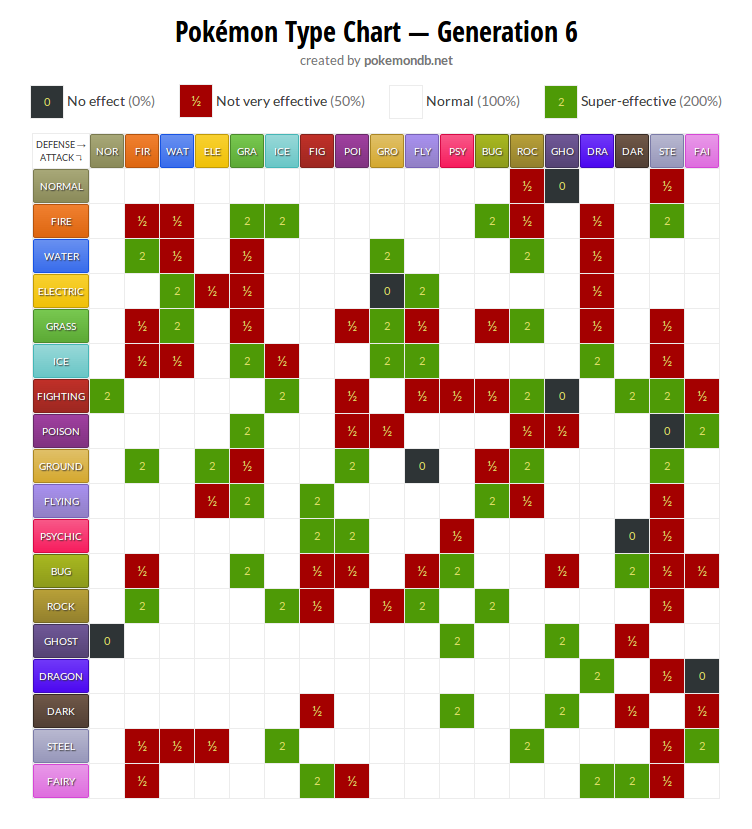
\includegraphics[width=0.85\textwidth]{img/typechart.png}
\caption{\label{fig:schema}Charte graphique des types, de leur forces et faiblesses, pokemondb.net/type}
\end{figure}

\subsubsection{Les statistiques du Pokémon}

Le Pokémon contient aussi des statistiques qui vont influencer sur ses dégâts infligés et subis et/ou sa viabilité en combat ou hors-combat. Dans cette section, nous allons décrire toutes les variables qui compose le Pokémon.

\begin{enumerate}
    \item Les points de vie
    
Un Pokémon a un nombre de point de vie maximale, qu'il ne peut pas dépasser. Si ses points de vie tombent à zéro, le Pokémon feint et n'est plus disponible pour se battre.

    \item L'Attaque
    
L'Attaque affecte les capacités physique du Pokémon. Elle intervient lors de l'affectation des points de dégâts infligés.

    \item L'Attaque Spécial
    
L'Attaque Spéciale affecte les capacités spéciale du Pokémon. Elle intervient lors de l'affectation des points de dégâts infligés.

    \item La Défense
    
La Défense affecte les capacités physique du Pokémon. Elle intervient lors de l'affectation des points de dégâts subis.

    \item La Défense Spéciale
    
La Défense Spéciale affecte les capacités spéciale du Pokémon. Elle intervient lors de l'affectation des points de dégâts subis.

    \item La Vitesse
    
La Vitesse détermine l'ordre d'action des Pokémons en combat. Sauf sous certaines exceptions, un Pokémon A dont la vitesse est supérieure à un Pokémon B attaquera en premier dans le tour.

    \item Les statistiques de base
    
Chaque Pokémon a des statistiques de base qui lui sont propres. Les statistiques notées ci-dessus peuvent fluctuer selon certains facteurs dont les statistiques de base du Pokémon concerné. Les statistiques de base ne changeront pas durant la progression du Pokémon.

    \item Les Points Individuelles - IV
    
Les points individuelles, ou IV, sont déterminées à la naissance du Pokémon ou lors de sa rencontre dans la nature. Les IV sont générées de manière dans chaque statistiques du Pokémon (Points de vie, Attaque, Attaque Spéciale, Défense, Défense Spéciale et Vitesse) et ils ne peuvent pas changer. Le total maximale des IV d'un Pokémon ne peut pas dépasser 186, et ne peut pas dépasser 31 d'IV par statistiques.

    \item Les Points d'Efforts - EV
    
Chaque fois qu'un Pokémon A bat un Pokémon B, le Pokémon A va recevoir un EV dans une statistique précise qui dépend du Pokémon B. Tout les 4 EV dans une statistique, la statistique augmente d'un point. En total, un Pokémon peut obtenir 510 EV, et 255 EV maximum dans une seule statistique.

\end{enumerate}

\subsubsection{La nature du Pokémon}

comportement lul truc qui te baisse une et te monte un

\subsubsection{Le talent du Pokémon}

Talent

\subsubsection{Les capacités du Pokémon}

Capacités
    Type
    Point de pouvoir - PP
    Degats
    Precision
    Effet
    Catégorie
        Capacité Physique
        Capacité Spéciale
        Capacité de statut
    Capacite Z
    
\subsubsection{Le statut du Pokémon}

Statut
    Principales
        Brulure
        Gel
        Paralisie
        Empoisonnement
        Sommeil
    Secondaires
        Attraction
        Confusion
        Malediction
        Peur
        Clairvoyance
        Vampigraine
        Piege
        Desobeissance
        
\subsubsection{L'esquive du Pokémon}

Esquive

\subsubsection{La forme du Pokémon}

Forme
    Permanente
    Combat
    En/Hors Combat
    
\subsubsection{Autres}

Poids

Bonheur
    

\subsection{Extérieur au Pokémon}

Climat
    Ensoleile
        Soleil intense
    Pluie
        Pluie batante
    Grele
    Tempete de sable
    Brouillard
    Souffle delta
Objets tenus
Objets dans le sac
    Hors-Combat
    En combat

\section{Format VGC}

Le tournoi
Définisse le format : 2vs2, etc
Le jeu utilisé
    -> Limite les pokémons utilisable
    -> Limite les capacités utilisable
    -> Limite les objets utilisable


\section{Pour notre goal}